% Upload mobilenetv1_kd_cosine_gradcampp.pdf; requires graphicx.
\begin{figure}[t]
  \centering
  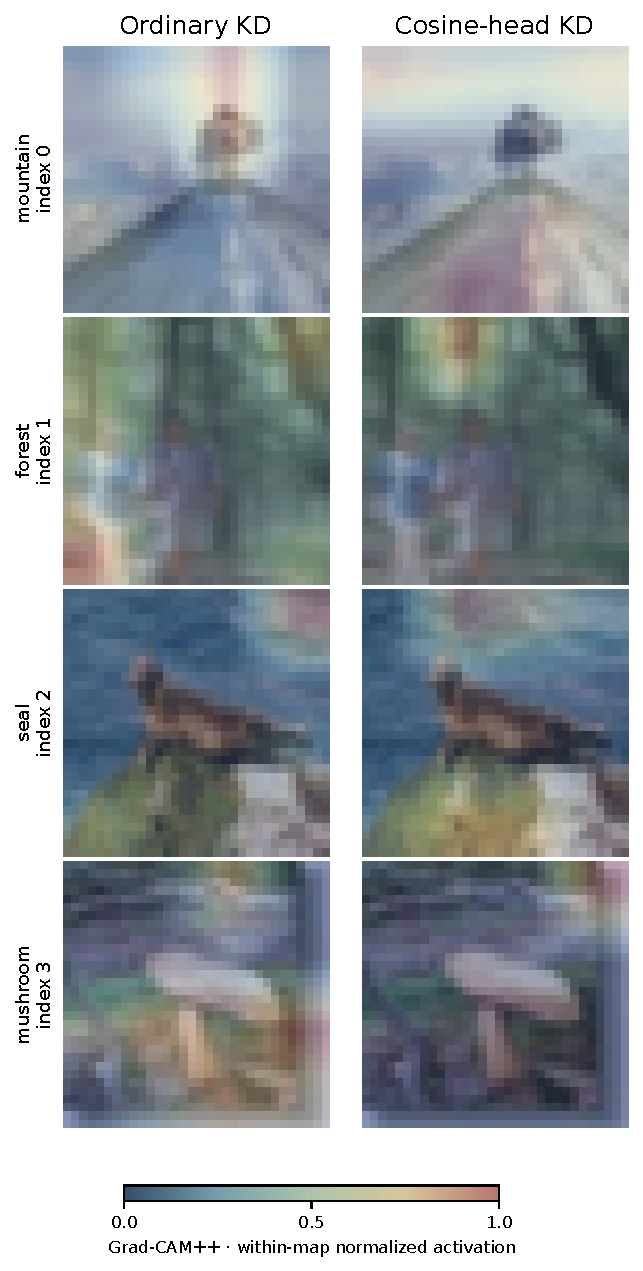
\includegraphics[width=\linewidth]{mobilenetv1_kd_cosine_gradcampp.pdf}
  \caption{\textbf{Grad-CAM++ comparison of trained MobileNetV1 models.}
  Columns compare ordinary KD and cosine-head KD with the same
  VGG13 teacher, seed 2051, and epoch-240 checkpoints on CIFAR-100.
  Rows are the first four official test images, fixed before attribution.
  Both models use the ground-truth class score as the attribution target.
  Maps use the same intermediate pointwise convolution (native $4\times4$),
  are bilinearly upsampled, independently min--max normalized, and blended
  with the input using fixed opacity and a shared color scale.
  Colors indicate relative spatial attribution, not comparable absolute
  gradient magnitude. Cosine-head KD is not the full ACI+SICD configuration.}
  \label{fig:gradcampp_kd_cosine}
\end{figure}
